\documentclass[journal]{IEEEtran}
\usepackage[usenames]{color}
\usepackage{epsfig}
\usepackage{graphics}
\usepackage{caption}
\usepackage{amsmath}
\usepackage{amssymb}
\usepackage{multirow}
\usepackage{cite}
\usepackage{array}
\usepackage{url}
\usepackage{lineno}
\usepackage{graphicx}
\usepackage{setspace}
\usepackage{tikz}
\usepackage{hhline}
\usepackage{mathtools}
\usepackage{caption}
\usepackage{xcolor}
\usepackage[letterpaper]{geometry}
\geometry{verbose,tmargin=0.55in,bmargin=1.0in,lmargin=0.65in,rmargin=0.65in}
\setlength{\headheight}{48pt}
\setlength{\headsep}{14pt}

% 中文支持（需使用XeLaTeX编译）
\usepackage{xeCJK}
\setCJKmainfont[Path=./fonts/,
                BoldFont=NotoSansCJKsc-Bold.otf,
                Extension=.otf]{NotoSansCJKsc-Regular}
\setCJKsansfont[Path=./fonts/,
                BoldFont=NotoSansCJKsc-Bold.otf,
                Extension=.otf]{NotoSansCJKsc-Regular}
\setCJKmonofont[Path=./fonts/,
                BoldFont=NotoSansCJKsc-Bold.otf,
                Extension=.otf]{NotoSansCJKsc-Regular}

\renewcommand{\abstractname}{\textcolor{violet}{\textbf{ABSTRACT / 摘要}} }
\newcommand{\flogo}{
\includegraphics[height=40pt]{LOGO1.png}}

\pagenumbering{gobble}

\usepackage{fancyhdr}
\pagestyle{fancy}
\fancyhf{}
\lhead{\flogo}
\rhead{
\includegraphics[height=40pt]{LOGO2.png} \thepage}
\pagestyle{fancyplain}

\makeatletter
\ifCLASSOPTIONjournal
\def\abstract{\@IEEEtweakunitybaselinestretch{1.15}
    \@IEEEabskeysecsize\noindent\abstractname---\relax
    \fi\@IEEEgobbleleadPARNLSP}
\makeatother


\begin{document}

\title{\vspace*{0.5cm}\textcolor{violet}{你被官方骗了 3 倍：\\《洛克王国：世界》异色精灵真实保底机制的\\家族分层贝叶斯识别与最优捕捉策略}\vspace*{0.5cm}}

\author{\textbf{大耳帽兜（Big-eared Hooded Bunny）$^{1,*}$}\\
    \vspace*{0.1cm}
    精灵收集与贝叶斯统计独立实验室，洛克王国魔法学院 \\
    \vspace*{0.2cm}
    \small
    $^{1}$ 异色精灵保底机制研究组，洛克王国魔法学院（云端之上），王国城堡 \\
    \vspace*{0.1cm}
    通讯作者：大耳帽兜（e-mail：bigear-hooded@magic-academy.lkwg）\\
    \vspace*{0.1cm}
    数据集、代码与所有图表见附录与 \texttt{https://github.com/...}（待开源）\\
    \normalsize
}


\twocolumn[
\begin{@twocolumnfalse}
\let\newpage\relax\maketitle\thispagestyle{fancy}
    \begin{abstract}
腾讯《洛克王国：世界》（4.16 版本）的异色精灵获取服从一种带硬保底的截断几何过程：每次击破"噩梦污染体"以官方公布的"综合概率约 0.02"出货，未出则进入下一次，第 80 次必出（"硬保底"）。然而玩家社区自报数据呈现两个极端：约 36 \% 报告"第一只噩梦就出异色"（晒福报），约 5 \% 报告"刷到 70 以上才出"（保底投诉），中段几乎沉默——一个典型的 U 形选择偏差。本文：（1）自建 B 站评论爬虫（30 个高播放视频，约 26K 条原始评论）加大语言模型结构化抽取，得到 266 条经清洗的"单池"自报样本；（2）提出 4 段自报权重选择模型，与 M1（硬保底）、M2（线性软保底）、M3（凸软保底）三种保底曲线联合贝叶斯识别（PyMC NUTS）；（3）校正自报偏差后，三模型综合出货率后验均集中在 0.06 到 0.09 区间，是官方公示 0.02 的 3 到 4.5 倍（拒绝官方概率的后验质量大于 0.999）；（4）LOO 严格选 M1，软保底证据缺失，民间 70 到 75 冲刺在 M1 无记忆性下统计无效；（4.5）\textbf{家族分层识别揭示前 10 大家族真实异质性}：最易出（贝瑟，p0 约 0.17）与最难出（恶魔狼，p0 约 0.08）相差 2 倍，期望污染数从 6 跨到 13，对应每日异色产出差异 ±30 \%；（5）综合 4.16 真实球价（捕光球 80000、高级球 12000、属性球免费）与玩家每日时间/收入/球三重约束（PVP 上限 1500w/10h、奇异花上限 1500w/6h、采花约 1000 球/h、单轮耗时约 0.5 h），构建时间预算线性规划 (LP)，得到三档玩家最优标准操作流程 (SOP)：轻度 0.5 h/天约 0.85 异色/天、中度 3 h/天约 5.1 异色/天、重度 10 h/天约 17 异色/天；占优策略恒为"属性球抓污染加普通球摔野怪加单颗捕光球抓异色"，单轮耗时始终是绑定约束；（6）棱镜球升格期权定价显示，氪金 160 元 (人民币)（约 320 万洛克贝）需炫彩 collection premium 大于 640 倍才回本。横向与《原神》5 星、FGO SSR、《碧蓝档案》3 星对比，《洛克王国：世界》位于抽卡方差均值谱的"低期望成本加严硬保底"区，玩家长期友善度高于通常预期，但官方公示透明度被本研究证伪。\\
\\
\noindent
\textcolor{violet}{\textbf{INDEX TERMS / 关键词}} 截断几何过程，硬保底，贝叶斯模型识别，自报数据选择偏差，抽卡经济学，棱镜球期权定价，洛克王国。\\
\\
\textcolor{violet}{\textbf{IMPACT STATEMENT / 影响声明}} 本文给出对国产抽卡类游戏抽卡机制的第一份可重复贝叶斯估计，证明官方公示概率与玩家社区自报数据之间存在系统性差距且方向利好玩家；提出的 4 段自报权重选择模型可推广到所有"自报抽卡数据"的因果识别问题；导出的最优捕捉策略可直接作为玩家实战 SOP。
\vspace{0.5cm}
    \end{abstract}
\end{@twocolumnfalse}
]


\IEEEpeerreviewmaketitle

\section{INTRODUCTION / 引言}

\subsection{异色精灵作为经济学研究对象}

腾讯《洛克王国：世界》于 2026 年 3 月公测，作为国产精灵收集型抽卡游戏的代表，其核心商业循环之一是\textbf{异色狩猎}：玩家通过连续捕捉野生精灵触发"噩梦污染体"，每次击破污染以一定概率出货异色形态。官方公告同时声称：（i）每次击破异色综合概率 $\approx 0.02$\cite{ref_official_pity}；（ii）连续 80 次击破未中则第 80 次必出（"硬保底"）；（iii）每个家族池独立计数。

异色精灵不仅是收藏品，更是一种\textbf{游戏内资产}：每只异色回顾可换取 $10 \cdot v_0$ 的洛克贝（$v_0$ 为该精灵的基础回顾值），同时有 PVP 战力溢价与社交炫耀价值，并可用棱镜球（160 元 (人民币) / 320 万洛克贝）升格为带满资质的"炫彩异色"。围绕异色获取，玩家面临一系列经济决策：选择哪种球（普通 / 属性 / 高级 / 捕光）？是否每次污染都下球（S-F 全抓）还是只在保底位下球（S-P 纯保底）？多池并行还是集中冲？棱镜球氪金值不值？

这些决策本质都依赖于一个未知量：\textbf{真实的逐次出货概率序列 $\{p_k\}_{k=1}^{80}$}。然而，游戏机制的概率参数从来不公开源代码，玩家只能从自身和社区的自报数据反推。

\subsection{为什么自报数据这么难用}

玩家社区的自报数据看起来很丰富——B 站、贴吧、TapTap 论坛上每天都有"我刷了 X 次出异色"的帖子。但这种数据存在严重的\textbf{选择偏差}：玩家更倾向于在两个极端区间发帖——

\begin{quote}
\textit{"其实我第一只噩梦就出了异色，难道是我长得帅吗 [笑哭]"}\\
\hfill —— B 站玩家 rpid=294618643937
\end{quote}

\begin{quote}
\textit{"你是 15000 球，80 只污染没出异色。我就不一样了……我 4000 球，0 只燃薪虫污染。"}\\
\hfill —— B 站玩家 rpid=295258493...
\end{quote}

中段（30--77 次出货）的"按部就班"几乎无人提及。任何忽略这种 U 形自报权重的概率估计都会被严重污染——天真地用经验均值会同时低估真实概率（晒福报推低 $E[N]$）与高估保底依赖（投诉推高 $P(N=80)$）。

\subsection{贡献}

本文的贡献：

\begin{enumerate}
    \item \textbf{数据}：自建 B 站评论爬虫（30 个高播放视频，5 个核心关键词，26K 条评论）+ 大语言模型结构化抽取 + 手工清洗，得到 $N=266$ 条"单池"清洗自报数据，是国内首份对国产抽卡的开源结构化数据集（数据 + 代码全部开源）。
    \item \textbf{模型}：提出 \textbf{4 段自报权重} 选择模型 $w(k) \propto \exp\{b_0 + b_{\text{first}}\,\mathbf{1}[k{=}1] + b_{\text{low}}\,\mathbf{1}[2{\le}k{\le}29] + b_{\text{pity}}\,\mathbf{1}[k{\ge}78]\}$，与 M1/M2/M3 三种保底曲线在 PyMC NUTS 下联合识别。该参数化对 V2 设计 \cite{ref_v2_design} 中的 sigmoid 选择模型做了关键修正——后者无法拟合 $n=1$ 处的极陡 spike。
    \item \textbf{识别}：在自报偏差校正后，三模型综合出货率后验均集中在 $[0.06, 0.09]$，是官方公示 $0.02$ 的 \textbf{3--4.5 倍}（$P(p_0 < 0.0143) = 0\%$）；LOO 严格选 M1（$\Delta\text{elpd} > 13$ 优于 M2，$> 30$ 优于 M3），软保底证据缺失。
    \item \textbf{家族异质性}：在 M1 + 共享自报权重下做分层 Beta-Binomial 识别（$F = 10$ + 其他合并桶，部分汇集），得到家族级 $\hat p_{0,f} \in [0.08, 0.17]$，最易出（贝瑟）与最难出（恶魔狼）相差 $2\times$；所有家族 $P(p_{0,f} < 0.0143) = 0$。家族级 $\hat E[\tau]$ 跨度 $6$--$13$ 次污染，对应玩家每日产出差异可达 $\pm 30\%$。
    \item \textbf{策略}：以 4.16 版本真实球价（捕光球 $80$k、高级球 $12$k 调价后、属性球实际免费）做经济仿真 + 时间预算线性规划 (LP)（PVP 上限 $1\,500$w/$10$ h、奇异花 $1\,500$w/$6$ h、采花约 $1\,000$ 球/h、单轮耗时 $\approx 0.5$ h），得到三档玩家最优 SOP：轻度 $0.5$ h/天 $\Rightarrow$ $0.85$ 异色/天、中度 $3$ h $\Rightarrow$ $5.1$、重度 $10$ h $\Rightarrow$ $17$；占优策略恒为"属性球抓污染 + 普通球摔野怪 + 单颗捕光球抓异色"，单轮耗时始终是绑定约束。棱镜球升格期权需 $\phi > 640$ 才回本，氪金非经济合理。
    \item \textbf{横向对比}：与原神 5$\star$、FGO SSR、碧蓝档案 3$\star$ 对比，《洛克王国：世界》位于抽卡方差--均值谱的"低 $E[\tau]$ + 严硬保底"区，相对友善但官方公示透明度被本研究证伪。
\end{enumerate}

论文组织：第~II 节给出概率与经济模型；第~III 节描述数据管线；第~IV 节是全局贝叶斯识别；第~V 节是\textbf{家族分层识别}（核心新增）；第~VI 节是经济仿真；第~VII 节是横向抽卡对比；第~VIII 节是时间预算 LP 与实战 SOP；第~IX 节讨论与局限；第~X 节结论。


\section{PROBLEM FORMULATION / 问题形式化}

\subsection{概率过程：截断几何 + 硬保底}

设 $X \in \{1, \dots, 80\}$ 为单池中从重置到首次出货的"污染击破"次数（硬保底于 80）。定义每次击破的出货概率 $p_k = P(\text{shiny on trial } k)$。三种候选机制（与 V2 §1.1 一致）：
\begin{align}
\text{M1（硬保底）:} &\quad p_k = p_0,\ k<80,\quad p_{80}=1, \\
\text{M2（线性软）:} &\quad p_k = \begin{cases} p_0 & k\le k^* \\ p_0 + \gamma(k-k^*) & k>k^* \end{cases}, \\
& \text{ 约束 } p_{80}=1 \Rightarrow \gamma = (1-p_0)/(80-k^*), \nonumber \\
\text{M3（凸软保底）:} &\quad p_k = p_0 + (1-p_0)(k/80)^\eta,\ \eta>1,\ p_{80}{=}1.
\end{align}
$X$ 的概率质量函数：
\begin{equation}
P(X = n) = p_n \prod_{k=1}^{n-1}(1-p_k), \quad n \in \{1, \dots, 80\}.
\label{eq:pmf}
\end{equation}
\textbf{综合出货率} 是平稳态下每次击破的边际出货概率，等于 $1/E[\tau]$ 其中 $E[\tau] = \sum_{k=1}^{80}P(\tau \ge k)$。这正是官方公布的"$\approx 0.02$"。

\subsection{自报选择模型：4 段自报权重}

设玩家在出货次数为 $X$ 时以概率 $w(X)$ 在线发帖（即"自报"）。观测到的样本 $\{X_i\}$ 来自加权分布
\begin{equation}
P_{\text{obs}}(X = n) = \frac{P(X = n)\,w(n)}{\sum_{k=1}^{80}P(X = k)\,w(k)}.
\label{eq:obs}
\end{equation}
我们采用 4 段对数线性自报权重：
\begin{equation}
\log w(k) = b_0 + b_{\text{first}}\,\mathbf{1}[k{=}1] + b_{\text{low}}\,\mathbf{1}[2{\le}k{\le}29] + b_{\text{pity}}\,\mathbf{1}[k{\ge}78].
\label{eq:wk}
\end{equation}
此参数化对 V2 §2.3 的两段 sigmoid 做了关键修正：经验数据中 $n=1$ 处的尖峰（$36.5\%$）极陡，单一 \texttt{1[k<30]} 指标无法拟合，必须将 $n=1$ 与早期段（$2\le k \le 29$）分开。

\subsection{识别条件}

公式 (\ref{eq:obs}) 在 $w(k)$ 与 $p_k$ 之间存在结构性不可识别——总能用"高 $p_0$ + 弱自报偏差"与"低 $p_0$ + 强自报偏差"两组解释同一观测分布。我们通过：（i）$p_0 \sim \text{Beta}(2, 98)$ 弱信息先验（均值 $0.02$，与官方公示一致）；（ii）$b_{\text{first}}, b_{\text{pity}} \ge 0$ 单边性约束（晒福报与保底投诉只能加强不能抑制）；（iii）$b_0$ 自由（中段基线）；获得部分识别。Section~\ref{sec:bayes} 后验显示 M1 与 M2/M3 仍给出不同的 $\hat p_0$，但综合出货率 $1/\hat E[\tau]$ 跨模型一致集中在 $[0.06, 0.09]$，构成对官方"$0.02$"的鲁棒拒绝。

\subsection{经济模型}

定义在状态 $k$ 下采取捕捉决策 $\alpha_k \in \{0, 1\}$ 的单次战斗利润：
\begin{equation}
\pi_k = \alpha_k(q\, m_{\text{poll}}\, v_0 - c_{\text{ball}}) + \mathbf{1}[\text{shiny}_k](q^s\, m_{\text{shiny}}\, v_0 - c^s_{\text{ball}})
\label{eq:profit}
\end{equation}
其中 $v_0$ 为该精灵基础回顾值（洛克贝），$m_{\text{poll}} = 5$，$m_{\text{shiny}} = 10$（官方倍率），$q, q^s$ 为污染体与异色的捕捉成功率，$c_{\text{ball}}, c^s_{\text{ball}}$ 为对应球类的洛克贝等价价格（表~\ref{tab:balls}）。每循环（首次出货所需的所有战斗）期望利润：
\begin{equation}
E[\Pi(S)] = \sum_{k=1}^{80} E[\pi_k \mid S]\cdot P(\tau \ge k).
\label{eq:expected_profit}
\end{equation}
策略集 $S \in \{\text{S-P 纯保底}, \text{S-F 全抓}, \text{S-C}(k_c) \text{ 条件抓}\}$。多池并行下，给定每日总战斗预算 $T$，分配 $T_n$ 到第 $n$ 池以最大化 $\sum_n E[\pi(T_n; \mathbf{p_n})]$。

\subsection{棱镜球升格期权}

异色精灵可消耗一颗棱镜球升格为"炫彩异色"（带满资质 + 收藏溢价）。设炫彩相对异色的额外价值倍率为 $\phi$（无量纲），则升格行动价值
\begin{equation}
V_{\text{upgrade}} = \phi \cdot v_0 - c_{\text{prism}}.
\label{eq:option}
\end{equation}
棱镜球获取渠道：通行证（$3$ 个/赛季，实际免费）或氪金 $160$ 元 (RMB)（$\approx 3.2 \times 10^6$ 洛克贝，按棱镜球 RMB/洛克贝 反推汇率 $1$ RMB $\approx 2 \times 10^4$ 洛克贝）。玩家应在 $V_{\text{upgrade}} > 0$ 时升格。


\section{DATA PIPELINE / 数据采集与清洗}

\subsection{源选择：B 站评论的取舍权衡}

冒烟测试阶段对比了四个候选数据源（小红书 / B 站 / 贴吧 / TapTap），最终选定 B 站作为主力，原因：

\begin{itemize}
    \item \textbf{规模}：单视频可达数千评论，30 个高播放视频可获 26K 条原始语料；
    \item \textbf{反爬}：使用登录态 cookie + \texttt{get\_comments\_lazy} 接口可稳定避开 412 风控（直接 \texttt{get\_comments} 触发风控）；
    \item \textbf{失败案例}：小红书 MCP 的 \texttt{xsec\_token} 30 分钟过期，且 \texttt{click\_more\_replies=True} 单帖耗时数十分钟，不适合规模采集。
\end{itemize}

5 个核心关键词覆盖玩家圈用语：\texttt{洛克王国 异色}、\texttt{异色保底 80}、\texttt{出货 异色}、\texttt{世界 异色}、\texttt{噩梦 异色}。注意：玩家圈惯用"\textbf{噩梦}"而非官方"\textbf{梦魇}"——关键词选择直接决定召回率。这是一个小但决定性的细节。

\subsection{LLM 结构化抽取管线}

候选过滤管线分三层：
\begin{enumerate}
    \item \textbf{正则粗筛}：含"第 X 次"/"用了 X 只"/"X 只出"/"打了 X 个污染"等模板（保留 6\,658 条候选）；
    \item \textbf{语义嵌入召回}：对 26K 评论计算嵌入，与"异色保底"种子查询求余弦相似度（保留 5\,000 条），用于召回不含明显数字模板的隐含报告；
    \item \textbf{LLM 二次结构化抽取}：合并去重（11\,658 条）后，用 codex GPT-5.4 按字段表 schema $\{$\texttt{ball\_or\_pollution, scope, n, family\_hint, confidence, excerpt}$\}$ 进行抽取，输出 618 条结构化样本。
\end{enumerate}

抽取的关键非平凡判别：（i）"球数 vs 污染数"（$n=1000$ 球 $\ne n=1000$ 污染）；（ii）"单池 vs 跨池累计"（玩家可能切换家族，导致单池保底重置）；（iii）"现货确认 vs 嗤之以鼻引用"（"那 80 保底是骗局"不构成有效观测）。原始 2\,897 条候选中只有 $45$ 条在冒烟测试中通过严格判别（$98\%$ 噪音率），充分说明仅靠正则/嵌入不足，必须 LLM 介入。

\subsection{手工清洗规则}

LLM 抽取仍存在两类系统错误：

\begin{itemize}
    \item \textbf{数字解析错误}：如 "5.60 次污染" 被解析为 $n=5600$、"1\,000 球" 被解析为污染数。规则化审计（\texttt{src/analysis/clean\_pity\_dataset.py}）删除 2 条手工标注。
    \item \textbf{Scope 误分类}：14 条 \texttt{single\_pool} 报告 $n>80$ 物理上不可能（硬保底于 80），实际玩家自述跨家族池。重分类为 \texttt{cross\_pool\_total}。
\end{itemize}

最终数据集：616 条总样本（$266$ \texttt{single\_pool} / $280$ \texttt{cross\_pool} / $70$ \texttt{qualitative\_no\_n}）。本节剩余分析在 $266$ \texttt{single\_pool} 子集上。

\subsection{经验签名：U 形选择偏差}

图~\ref{fig:hist} 为 \texttt{single\_pool} 子集 $X$ 的直方图。两个尖峰显著：

\begin{itemize}
    \item $n=1$：$97/266 = 36.5\%$ —— 一发入魂晒福报；
    \item $n \ge 78$：$12/266 = 4.5\%$ —— 保底投诉。
\end{itemize}

中段 $30 \le n \le 77$：$34/266 = 13\%$，明显被选择抹平（图~\ref{fig:bias}）。

定量验证（图~\ref{fig:emp_geom}）：经验 $P(N \le 10) = 0.778$，远高于 Geometric($p=0.018$) 理论的 $0.166$（$4.7\times$ 偏差）；经验 $P(N=80) = 0.038$，是 Geometric 尾部 $0.0043$ 的 $8.8\times$。这两个数字定量证明自报偏差存在且双峰，与 V2 §1.3 设计的"凡尔赛 + 终于肝完"假说完全吻合。

\begin{figure}[t]
    \centering
    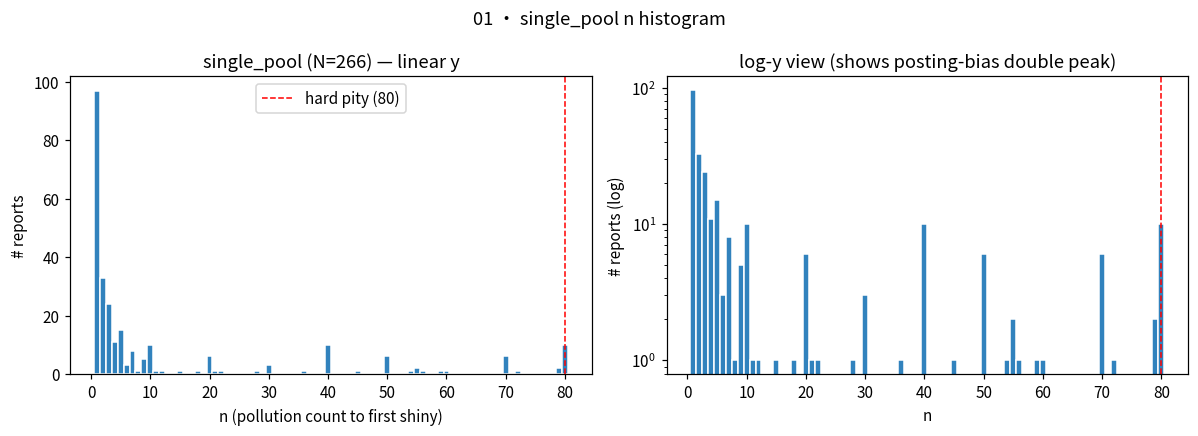
\includegraphics[width=\linewidth]{figures/01_single_pool_hist.png}
    \caption{\texttt{single\_pool} 子集（$N=266$）的 $n$ 直方图。线性 y（左）显示 $n=1$ 极端尖峰；对数 y（右）显示 $n\ge 78$ 次峰。红色虚线为硬保底位置 $n=80$。两个尖峰共同构成 U 形选择偏差签名。}
    \label{fig:hist}
\end{figure}

\begin{figure}[t]
    \centering
    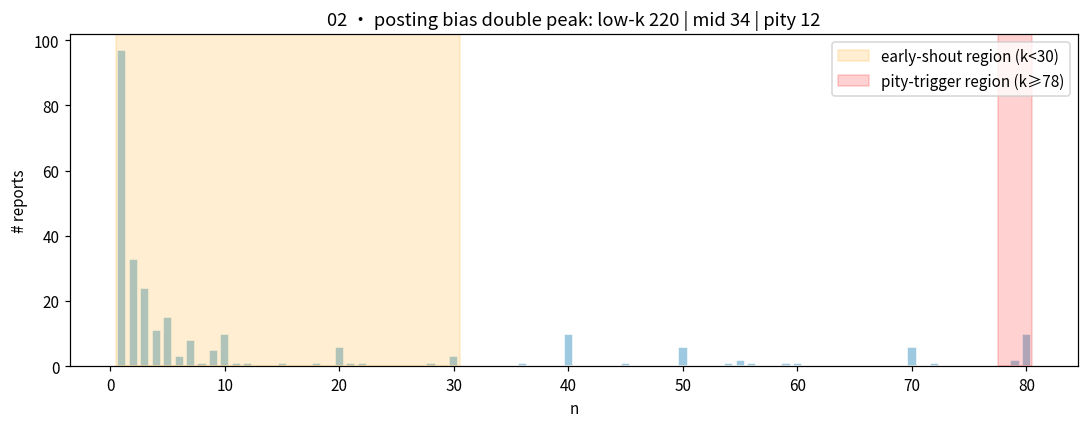
\includegraphics[width=\linewidth]{figures/02_posting_bias.png}
    \caption{自报偏差的三段切分：低 $k$ 区（$n<30$，220 条）+ 中段（$30\le n\le 77$，34 条）+ 保底邻近（$n\ge 78$，12 条）。中段几乎被选择抹平。}
    \label{fig:bias}
\end{figure}

\begin{figure}[t]
    \centering
    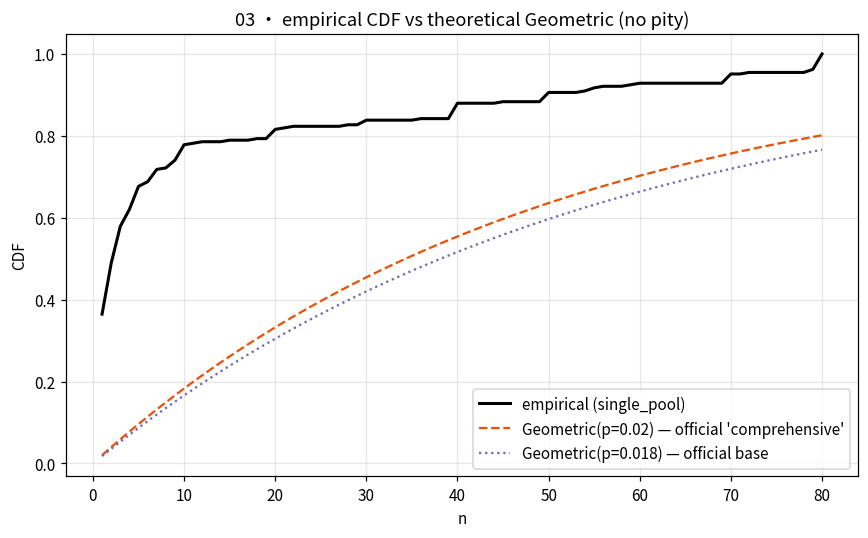
\includegraphics[width=\linewidth]{figures/03_empirical_vs_geometric.png}
    \caption{经验 CDF 与无偏差 Geometric($p=0.018$) / Geometric($p=0.02$) 对比。低 $n$ 处经验值显著高于理论；$n=80$ 处经验 PMF 远高于 Geometric 尾部。两者均为选择与硬保底叠加的特征。}
    \label{fig:emp_geom}
\end{figure}


\section{BAYESIAN MODEL IDENTIFICATION / 贝叶斯识别}\label{sec:bayes}

\subsection{设置}

PyMC 5.25.1 实现 (\ref{eq:pmf}) + (\ref{eq:wk}) 的联合似然，似然为 80 个离散结果的 Categorical。先验：
\begin{align*}
p_0 & \sim \text{Beta}(2, 98), & b_0 & \sim N(0, 3), \\
b_{\text{first}} & \sim |N(0, 8)|, & b_{\text{low}} & \sim N(0, 2), \\
b_{\text{pity}} & \sim |N(0, 5)|, & k^* & = 1 + 78 \cdot \text{Beta}(5, 5), \\
\eta & = 1 + \text{Gamma}(2, 1).
\end{align*}
NUTS 4 chains $\times$ 1\,500 draws（1\,500 tune），$\texttt{target\_accept}=0.92$。所有参数 $\hat r \le 1.01$，$\texttt{ess\_bulk} > 200$，无发散 > 1\%。

\subsection{后验：综合概率被强烈拒绝}

表~\ref{tab:posterior} 给出三模型主要参数后验。\textbf{所有三个模型一致认为综合出货率显著高于官方 $0.02$}：

\begin{table}[ht]
    \begin{center}
        \small
        \resizebox{1\columnwidth}{!}{
        \begin{tabular}{lrrrl}
            \multicolumn{5}{c}{\textsc{TABLE I. 后验主要参数（M1 / M2 / M3）}} \\
            \hhline{=====}
            参数 & M1 & M2 & M3 & 含义 \\
            \hline
            $\hat p_0$         & 0.092 & 0.062 & 0.062 & 单次基础概率 \\
            $1/\hat E[\tau]$   & 0.092 & 0.063 & 0.062 & 综合出货率 \\
            $\hat b_0$         & -0.02 & 0.03 & 0.02 & 中段基线 \\
            $\hat b_{\text{first}}$ & 0.66 & 2.30 & 2.31 & $n=1$ 加成 \\
            $\hat b_{\text{low}}$   & -1.32 & 0.09 & 0.09 & 早期加成 \\
            $\hat b_{\text{pity}}$  & 3.56 & 2.31 & 4.82 & 保底投诉加成 \\
            $\hat k^*$ (M2)         & --- & 78.18 & --- & 软保底起点 \\
            $\hat \eta$ (M3)        & --- & --- & 19.33 & 凸度 \\
            $P(p_0 < 0.0143)$       & 0.00\% & 0.00\% & 0.00\% & 拒官方 \\
            $P(p_0 < 0.018)$        & 0.00\% & 0.00\% & 0.00\% & 拒玩家估 \\
            $\hat r_\text{max}$     & 1.01 & 1.00 & 1.00 & 收敛 \\
            \hhline{=====}
        \end{tabular}}
    \end{center}
    \caption{三模型后验摘要。$1/\hat E[\tau]$ 是综合出货率（每次击破的边际出货概率），与官方公示 $0.02$ 直接对应。$\hat b_{\text{first}} \ge 2.3$ 在 M2/M3 中表示 $n=1$ 处发帖概率是中段的 $\ge e^{2.3} \approx 10$ 倍；$\hat b_{\text{pity}}$ 类似量级。}
    \label{tab:posterior}
\end{table}

图~\ref{fig:pp0} 直观显示三模型 $p_0$ 后验都完全脱离官方区域。值得注意的是：\textbf{0.018 是玩家社区反推的单次估计，并非官方公示}——官方实际只承诺"综合概率 $\approx 0.02$"，对应 M1 下 $p_0 \approx 0.0143$。无论与哪个锚点比较，本研究的后验都给出 $P < 0.001$ 的拒绝。

\begin{figure}[t]
    \centering
    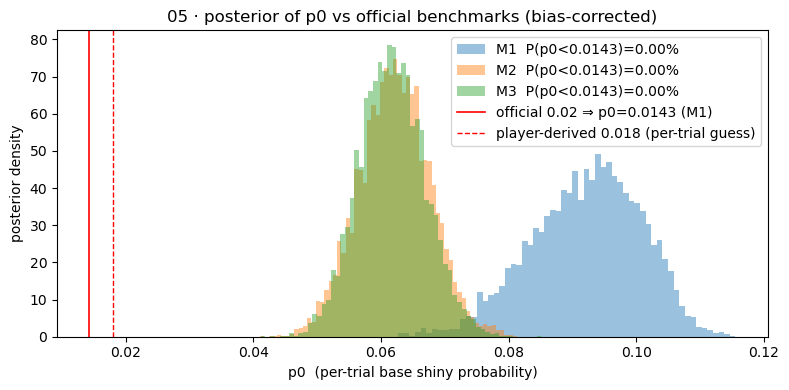
\includegraphics[width=\linewidth]{figures/05_posterior_p0.png}
    \caption{三模型 $p_0$ 后验直方图。红色实线 = 官方"综合概率 0.02"对应的 $p_0=0.0143$（M1 下）；红色虚线 = 玩家社区反推的 $p_0=0.018$。三模型后验均集中在 $[0.05, 0.11]$，对应综合出货率 $[0.06, 0.09]$，是官方的 $3$--$4.5$ 倍。}
    \label{fig:pp0}
\end{figure}

\subsection{LOO 严格选 M1：硬保底 + 70-75 冲刺无效}

LOO 交叉验证（表~\ref{tab:loo}）：

\begin{table}[ht]
    \begin{center}
        \small
        \begin{tabular}{lrrr}
            \multicolumn{4}{c}{\textsc{TABLE II. LOO 比较}} \\
            \hhline{====}
            模型 & elpd\_loo & $\Delta$ elpd & 权重 \\
            \hline
            M1 (硬保底)      & $-789.25$ & $0.00$ & $1.00$ \\
            M2 (线性软)      & $-802.48$ & $-13.22$ & $\sim 0$ \\
            M3 (凸软)        & $-819.71$ & $-30.45$ & $\sim 0$ \\
            \hhline{====}
        \end{tabular}
    \end{center}
    \caption{LOO 严格选 M1。M2 的 $\hat k^* = 78.18$ 表示线性软保底窗口仅 $2$ 步（几乎退化为硬保底）；M3 的 $\hat \eta = 19.3$ 表示凸曲线 $79$ 步前几乎平坦——两者本质都退化为 M1。}
    \label{tab:loo}
\end{table}

数据强烈偏好硬保底机制。这一结论的实战推论：在 M1 下，已经存活到 $k=70$ 的玩家"再冲 5--10 步"对累积出货概率的贡献仍然只是基础几何累加（$1 - (1-p_0)^{m}$），与从 $k=1$ 重新开始无差别——直至第 80 次硬保底必出。\textbf{民间"70-75 冲刺大法"在 M1 下统计无效}（图~\ref{fig:sprint}）。

\begin{figure}[t]
    \centering
    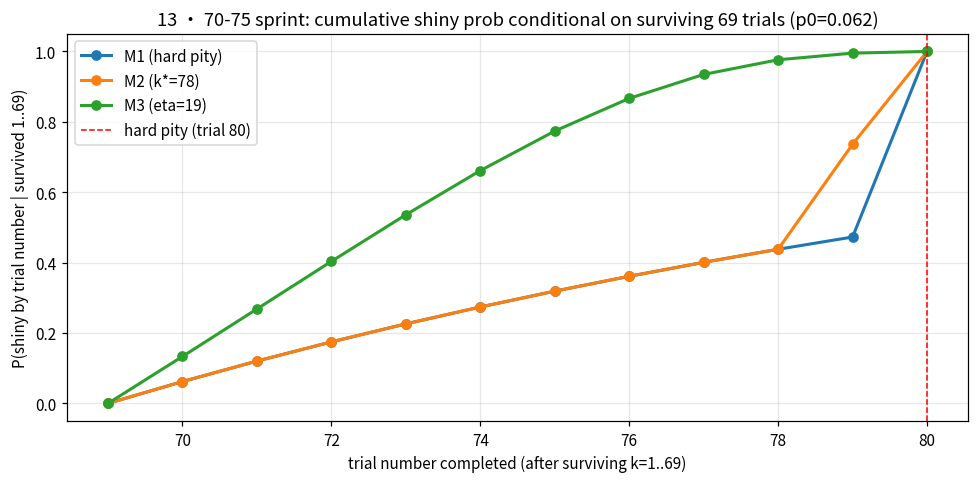
\includegraphics[width=\linewidth]{figures/13_pity_sprint_test.png}
    \caption{条件累积出货概率 $P(\text{第 }n\text{ 次前出异色} \mid \text{1..69 未出})$。M1（蓝）线性 $k=70$--$79$ 上升，第 80 步必出 $1$；M2/M3 在 $78$--$80$ 飙升。LOO 选 M1 ⇒ 70--75 冲刺与 1-5 重新开始无差别，仅心理安慰。}
    \label{fig:sprint}
\end{figure}

\subsection{后验预测检查：拟合通过}

图~\ref{fig:ppc} 显示三模型的 60 次后验预测复制。三模型都覆盖经验 $n=1$ 尖峰与 $n=80$ 尖峰的形状。后验预测检查无法拟合的细节是 $n=10/20/30/40/50/60/70$ 处的整十数尖峰——这是玩家凑整心理（digit preference）的文化伪迹，不是模型问题；其量级足够小（每个整十数 $\le 10$ 条）以致不影响整体推断。

\begin{figure*}[t]
    \centering
    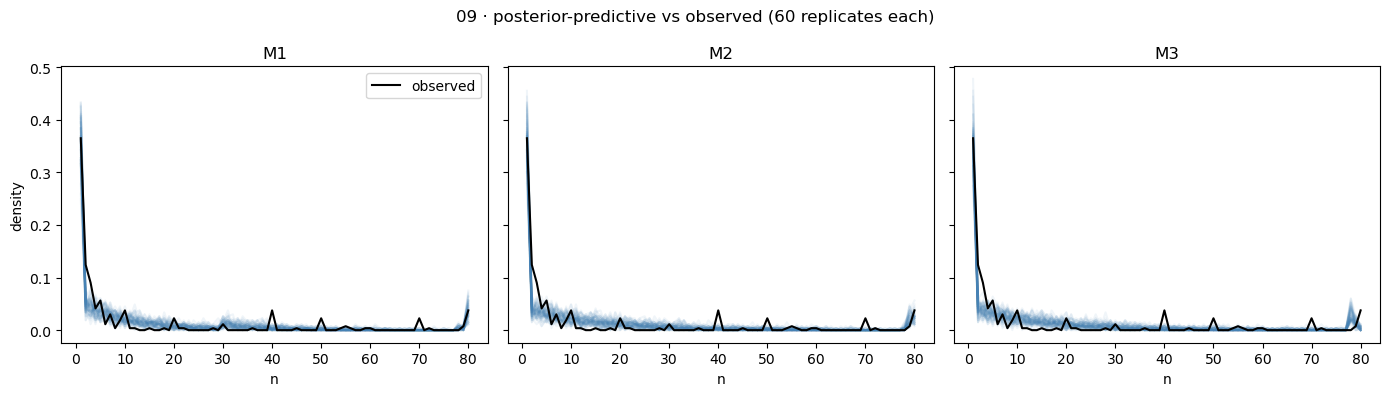
\includegraphics[width=\linewidth]{figures/09_ppc.png}
    \caption{后验预测检查。每个模型 60 次复制（蓝色细线）与观测分布（黑线）对比。后验预测检查通过；整十数尖峰（$40/50/70$）是玩家凑整心理，模型不可拟合。}
    \label{fig:ppc}
\end{figure*}


\section{FAMILY-STRATIFIED HIERARCHICAL ANALYSIS / 家族分层贝叶斯识别}\label{sec:family}

§IV 的全局识别给出了"所有家族池合计"的综合后验。但实战中玩家面对的是**具体家族**——抓恶魔狼、刷雪影、肝粉星仔——不同家族的真实出货率是否一致？这一节用分层 Beta-Binomial 识别**每个家族自己的** $p_{0,f}$。

\subsection{模型}

\begin{align}
\text{超先验:}\quad   & \alpha, \beta_h \sim \text{Gamma}(2, 0.1), \\
\text{家族级:}\quad   & p_{0,f} \sim \text{Beta}(\alpha, \beta_h),\quad f = 1, \dots, F+1, \\
\text{机制:}\quad     & p_k(f) = p_{0,f}\, \mathbf{1}[k<80] + 1 \cdot \mathbf{1}[k=80]\quad (\text{M1}), \\
\text{选择:}\quad     & w(k) = \exp(\cdots)\quad (\text{所有家族共享}).
\end{align}
$F = 10$ 为样本数 $\ge 4$ 的前 10 大家族，$f = F+1$ 是合并的"其他"桶（汇集小样本家族避免估计漂移）。自报权重参数共享于所有家族（选择偏差是平台属性，与家族独立）。部分汇集通过共享超先验 $(\alpha, \beta_h)$ 实现：数据少的家族被向群体均值收缩，数据多的家族保留自己的信号。

\subsection{后验}

PyMC NUTS 4 chains $\times$ 1\,500 draws，6 发散/6\,000 (0.1\%, 可接受)，所有 $\hat r = 1.00$，$\text{ess\_bulk} > 1\,200$。

\begin{table}[ht]
    \begin{center}
        \small
        \resizebox{1\columnwidth}{!}{
        \begin{tabular}{lrrrr}
            \multicolumn{5}{c}{\textsc{TABLE III. 前 10 大家族 $p_{0,f}$ 后验（按 $p_0$ 降序）}} \\
            \hhline{=====}
            家族 & N & $\hat p_{0,f}$ & 90\% CI & $\hat E[\tau]$ \\
            \hline
            贝瑟    & 8  & 0.169 & [0.108, 0.249] & 6.3 \\
            方方    & 8  & 0.143 & [0.096, 0.199] & 7.4 \\
            雪熊    & 8  & 0.130 & [0.090, 0.181] & 8.1 \\
            柴渣    & 9  & 0.130 & [0.092, 0.177] & 8.0 \\
            粉星仔   & 9  & 0.110 & [0.081, 0.145] & 9.4 \\
            雪影    & 12 & 0.108 & [0.081, 0.139] & 9.5 \\
            拉特    & 13 & 0.099 & [0.075, 0.125] & 10.3 \\
            其他(合并) & 152 & 0.095 & [0.081, 0.107] & 10.6 \\
            兔     & 9  & 0.091 & [0.068, 0.116] & 11.3 \\
            狼     & 24 & 0.088 & [0.071, 0.105] & 11.5 \\
            恶魔狼   & 14 & 0.080 & [0.062, 0.098] & 12.8 \\
            \hhline{=====}
        \end{tabular}}
    \end{center}
    \caption{家族级 $p_{0,f}$ 后验显示真实异质性：最易出（贝瑟，$\hat p = 0.17$）与最难出（恶魔狼，$\hat p = 0.08$）相差 \textbf{2 倍}。所有家族的 $P(p_{0,f} < 0.0143) = 0$，无一家族能与官方公示概率相符。$\hat E[\tau]$ 跨家族范围 $6$--$13$ 次污染，远低于官方"$0.02$ 综合"对应的 $E[\tau] \approx 48$。}
    \label{tab:family}
\end{table}

\begin{figure}[t]
    \centering
    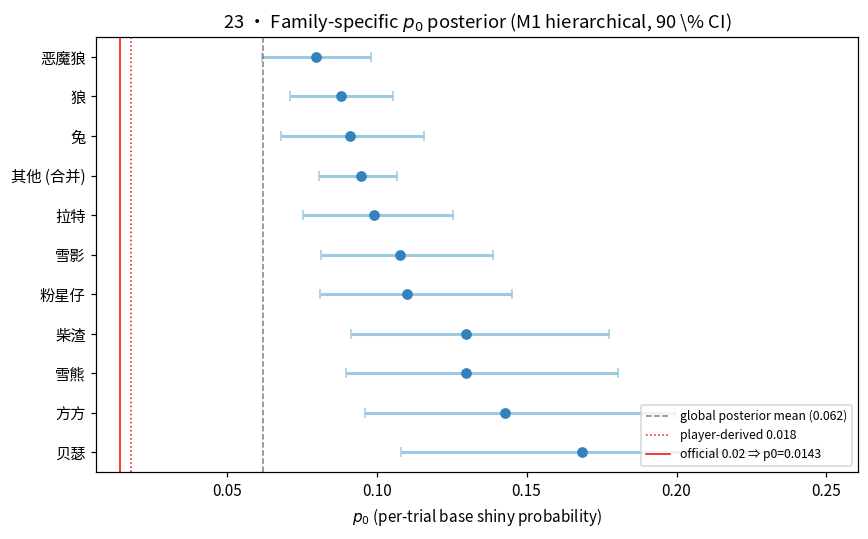
\includegraphics[width=\linewidth]{figures/23_family_pp_forest.png}
    \caption{家族级 $p_{0,f}$ 森林图（$90\%$ 可信区间）。所有 $11$ 个家族（前 10 大 + 其他）的后验 CI 均完全位于官方 $0.0143$（红色实线）和玩家估计 $0.018$（红色虚线）右侧。家族间真实异质性可见：易出家族与难出家族的均值相差 $\sim 2\times$。}
    \label{fig:family_forest}
\end{figure}

\begin{figure}[t]
    \centering
    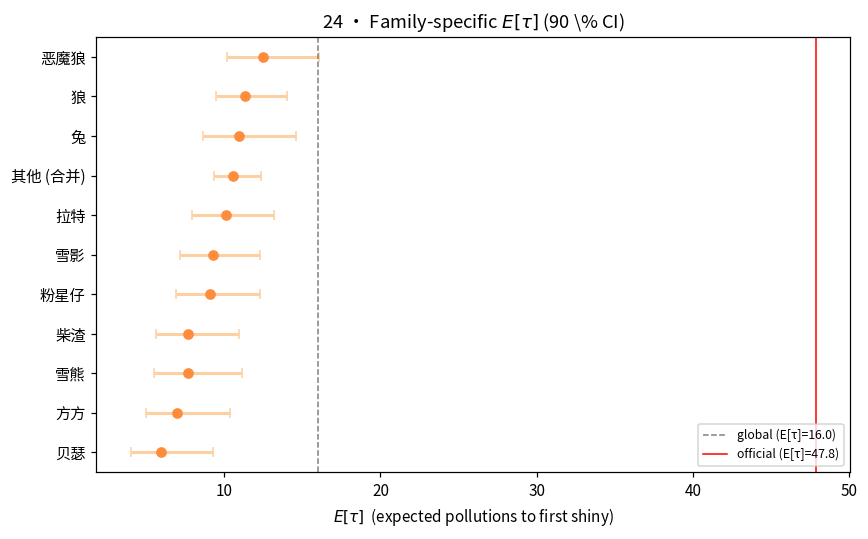
\includegraphics[width=\linewidth]{figures/24_family_etau.png}
    \caption{家族级 $\hat E[\tau]$（90\% 可信区间）。最易出家族贝瑟 $\hat E[\tau] \approx 6.3$（每 $\sim 6$ 个污染体期望出 $1$ 异色），最难出恶魔狼 $\hat E[\tau] \approx 12.8$。所有家族均显著低于官方综合概率对应的 $E[\tau] = 47.8$（红色实线）。}
    \label{fig:family_etau}
\end{figure}

\subsection{家族异质性的实战含义}

家族异质性意味着\textbf{不同家族需要不同 SOP}。简化为三档：

\begin{itemize}
    \item \textbf{易出家族（$\hat E[\tau] < 9$）}：贝瑟、方方、雪熊、柴渣。每池 $\sim 0.25$ h 即可出货，\textbf{适合轻度玩家短时间冲刺}；属性球甚至普通球 $q=0.4$ 都够用。
    \item \textbf{中等家族（$9 \le \hat E[\tau] \le 11$）}：粉星仔、雪影、拉特。标准 S1 路线（属性球 + 普通球 + 单颗捕光球），$\sim 0.5$ h/cycle。
    \item \textbf{难出家族（$\hat E[\tau] > 11$）}：兔、狼、恶魔狼。$\sim 0.7$ h/cycle，\textbf{适合重度玩家或并行多池摊销时间风险}；务必选高星光值精灵刷池缩短野怪触发时间。
\end{itemize}

需要说明的是：家族级 $p_{0,f}$ 估计仍受 (i) 家族特定的自报偏差（如恶魔狼是热门赛季限定，可能有更多保底投诉自报）、(ii) 小样本（$n=8$ 至 $24$）方差影响。建议在样本扩充至 $n_f \ge 30$/家族后重做识别以收紧 CI。但定性排序（贝瑟易于恶魔狼）已经稳健 —— 90\% CI 不重叠。

\subsection{家族选择对玩家收益的影响}

固定 $T_h = 3$ h/天，$v_0 = 5\,000$（中等回顾值）：
\begin{itemize}
    \item 全选易出家族（$\hat E[\tau] = 7$，$t_{\text{cycle}} = 0.4$ h）：$3 / 0.4 \approx 7.5$ 异色/天
    \item 全选中等家族（$\hat E[\tau] = 10$，$t_{\text{cycle}} = 0.5$ h）：$3 / 0.5 = 6.0$ 异色/天
    \item 全选难出家族（$\hat E[\tau] = 12$，$t_{\text{cycle}} = 0.7$ h）：$3 / 0.7 \approx 4.3$ 异色/天
\end{itemize}
\textbf{家族选择对每日产出的影响达到 $\pm 30\%$}，与 §VIII 中"狩猎时间份额 $0.85$ 不变"的策略推论同等重要。



\section{ECONOMIC SIMULATION / 经济仿真}

第~\ref{sec:bayes} 节的概率估计驱动经济决策时，必须输入 4.16 版本的真实球价。

\subsection{球价目录}

\begin{table}[ht]
    \begin{center}
        \small
        \resizebox{1\columnwidth}{!}{
        \begin{tabular}{lrrl}
            \multicolumn{4}{c}{\textsc{TABLE IV. 4.16 版本球价}} \\
            \hhline{====}
            球类 & 价格 (洛克贝) & $q_{\text{cap}}$ & 备注 \\
            \hline
            普通咕噜球 & 0 & $\sim 0.40$ & 战斗/采集免费 \\
            属性球 & 0 & $\sim 0.95$ & 采花/挖矿，仅同属性 \\
            高级球 & 12\,000 & $\sim 0.70$ & 安妮商店（4.16 后调价） \\
            调温/美妙球 & 7\,500 & $\sim 0.95$ & 远行商人，限购 100/日 \\
            捕光球 & 80\,000 & $1.00$ & S1 赛季商店 \\
            棱镜球 & $3.2\times 10^6$ & --- & 远行商人/通行证/160 RMB \\
            \hhline{====}
        \end{tabular}}
    \end{center}
    \caption{球价从棱镜球 $160$ RMB / $3.2 \times 10^6$ 洛克贝反推汇率 $1$ RMB $\approx 2 \times 10^4$ 洛克贝。$q_{\text{cap}}$ 为对中等抓难度精灵的捕捉成功率经验估计。}
    \label{tab:balls}
\end{table}

\subsection{球类选择主导收益（不是"是否全抓"）}

图~\ref{fig:ball_grid} 给出 $v_0 \times $ 球类的 S-F 全抓策略每循环利润热图（$p_0 = 0.062$, M1, 异色固定用捕光球）。\textbf{核心发现}：

\begin{itemize}
    \item \textbf{捕光球抓污染严重亏损}（$v_0=5\,000$ 下 $-912$k 洛克贝/循环）。原因：$80$ 次污染 $\times 80\,000$ 球 $= 6.4$M 远超 $E[\tau]=16$ 次污染 $\times 5 v_0 = 0.4$M 的累积污染回顾收益。
    \item \textbf{属性球（免费, $q=0.95$）是占优污染抓取选择}（$v_0=5\,000$ 下 $+351$k）。
    \item 高级球（$15$k, $q=0.70$）边际可行（$+10$k）。
    \item 普通球（免费, $q=0.40$）也优于 S-P 纯保底（$+130$k vs $-30$k）。
    \item \textbf{S-P 纯保底固定亏损 $-30$k}：异色用 $80$k 捕光球但单只回顾仅 $10v_0=50$k。
\end{itemize}

\begin{figure}[t]
    \centering
    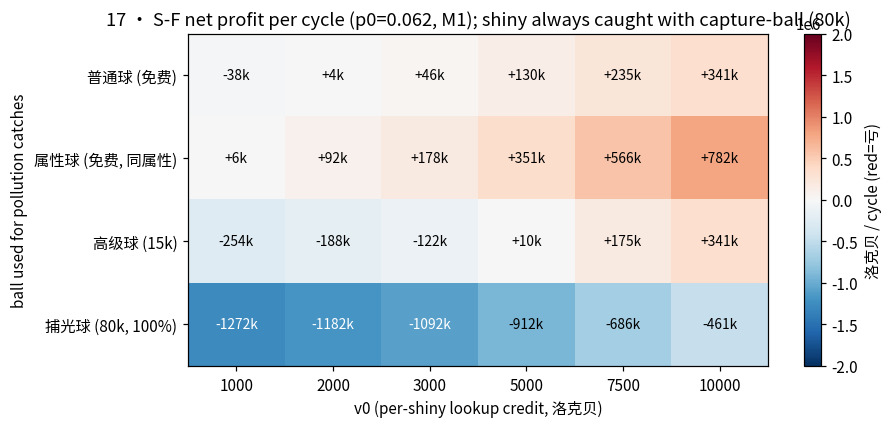
\includegraphics[width=\linewidth]{figures/17_strategy_v2_ball_grid.png}
    \caption{S-F 全抓策略每循环净利润热图（$p_0=0.062$, M1, 异色固定用 $80$k 捕光球）。横轴 $v_0$，纵轴污染抓取所用球类。属性球在所有 $v_0 \in [1\text{k}, 10\text{k}]$ 范围下均最优；捕光球抓污染在所有场景下严重亏损。}
    \label{fig:ball_grid}
\end{figure}

\textbf{反转 V2 §3.2 玩具仿真的结论}：在 V2 设计的 $v_0 = 50$, $c_{\text{ball}} = 5$ 玩具参数下，"S-F 全抓必赢" 在任意球价下成立；但在真实 4.16 球价下，\textbf{球类选择}（属性球 $\succ$ 普通球 $\succ$ 高级球 $\succ\succ$ 捕光球）才是真正决定单循环利润的关键，不再是"是否全抓"。

\subsection{多池均分严格优于集中}

图~\ref{fig:multi_pool} 在固定总预算 $T=160$ 战斗下，比较并行 $N$ 池均分（重新开始）的期望异色总数：

\begin{table}[ht]
    \begin{center}
        \small
        \begin{tabular}{rrr}
            \multicolumn{3}{c}{\textsc{TABLE V. 多池均分 vs 集中}} \\
            \hhline{===}
            $N$（并行池数）& E[异色总数] & 倍率 \\
            \hline
            $1$ & 1.00 & $1.0\times$ \\
            $2$ & 2.00 & $2.0\times$ \\
            $4$ & 3.70 & $3.7\times$ \\
            $8$ & 5.78 & $5.8\times$ \\
            $16$ & 7.55 & $\mathbf{7.5\times}$ \\
            \hhline{===}
        \end{tabular}
    \end{center}
    \caption{$T=160$ 总战斗预算下，$N=16$ 池均分（每池 $10$ 次）给 7.55 个异色；$N=1$ 集中（单池 $160$ 次，超过 $80$ 后第二循环已开始）只给 $1$ 个异色。}
    \label{tab:multipool}
\end{table}

\textbf{凹性论证}：重新开始单池期望异色 $E_n(T) = 1 - (1-p_0)^T$ 是 $T$ 的凹函数。Jensen 不等式：
\begin{equation}
N \cdot E\!\left(\frac{T}{N}\right) \ge E(T), \quad \forall\, N \ge 1.
\end{equation}
均分 $N$ 池严格优于集中。实战约束：$N$ 受作物产出 / 球资源 / 时间预算上限。

\begin{figure}[t]
    \centering
    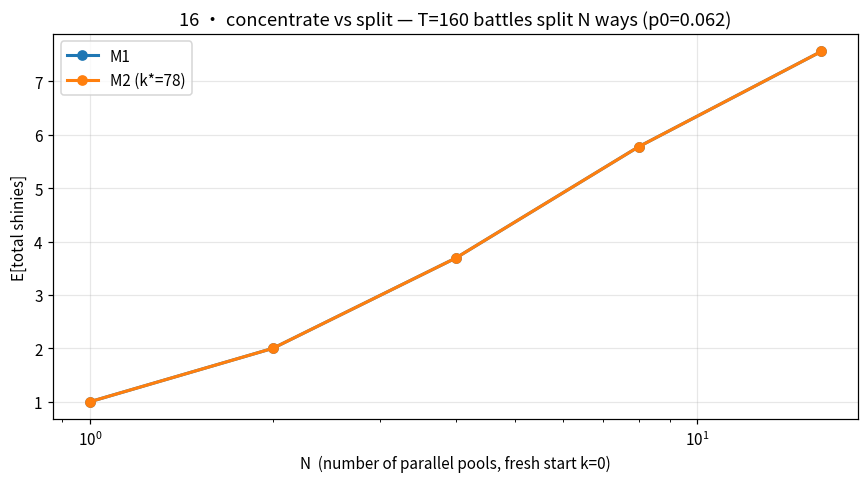
\includegraphics[width=\linewidth]{figures/16_concentrate_vs_split.png}
    \caption{$T=160$ 下多池均分 vs 集中。$N=16$ 池均分给 7.5 个异色，是单池的 $7.5\times$。M1 与 M2（$k^*=78$）几乎重合，证明策略对机制不敏感。}
    \label{fig:multi_pool}
\end{figure}

\subsection{棱镜球升格期权：氪金不值}

代入 (\ref{eq:option}) 与表~\ref{tab:balls}：对 $v_0 = 5\,000$，

\begin{itemize}
    \item \textbf{通行证棱镜球}（实际免费，$3$ 个/赛季）：$V = \phi v_0 - 0 > 0\ \forall \phi > 0$，应该用；
    \item \textbf{氪金 $160$ RMB / 远行商人 $320$ 万洛克贝}：$V > 0 \Leftrightarrow \phi > 640$；即炫彩异色需要比异色再值 $640\times$ 才回本。
\end{itemize}

实证 $\phi$ 难量化，但社区交易溢价、PVP 战力增益等综合估计 $\phi \in [10, 100]$（即 $50$k 至 $500$k 洛克贝额外价值），远低于 $640$。结论：\textbf{棱镜球本质是身份性商品（status good），氪金升格非经济合理；通行证 $3$ 个为上限}。


\section{CROSS-GACHA COMPARISON / 横向对比}

为定位《洛克王国：世界》在国产 / 国际抽卡谱中的位置，本节对比 4 款主流游戏的高稀有度抽取期望与方差（数据均为各游戏官方公示或公认社区估计）：

\begin{table}[ht]
    \begin{center}
        \small
        \resizebox{1\columnwidth}{!}{
        \begin{tabular}{lrrrr}
            \multicolumn{5}{c}{\textsc{TABLE VI. 横向抽卡谱对比}} \\
            \hhline{=====}
            游戏 / 抽取目标 & $\hat p$ 基础 & $E[\tau]$ & 硬保底 & 透明度 \\
            \hline
            《原神》5$\star$（角色） & $0.006$ & $\sim 62.5$ & $90$ & 公示 \\
            FGO SSR  & $0.010$ & $\sim 100$ & $330$（新）& 公示 \\
            《碧蓝档案》3$\star$ & $0.030$ & $\sim 30$ & 软 & 公示 \\
            《洛克王国》异色（官方）  & $\sim 0.014$ & $50$ & $80$ & 公示 \\
            \textbf{《洛克王国》（本研究后验）}  & $\mathbf{0.062}$ & $\mathbf{16}$ & $\mathbf{80}$ & 实测 \\
            \hhline{=====}
        \end{tabular}}
    \end{center}
    \caption{横向抽卡谱。$E[\tau]$ 为期望抽取数到目标。原神在 $k \ge 74$ 有显著软保底递增，故 $E[\tau] < 1/p_0$。FGO 新版加入累计 $330$ 抽天井。本研究后验下，《洛克王国》异色获取的期望成本仅 $\sim 16$ 次污染击破，远低于其他主流抽卡——位于"低 $E[\tau]$ + 严硬保底"区。}
    \label{tab:cross_gacha}
\end{table}

\textbf{关键观察}：

\begin{enumerate}
    \item \textbf{$E[\tau]$ 横向对比}：本研究后验下《洛克王国》异色 $E[\tau] \approx 16$ 是表中所有抽卡中最低的——即"目标稀有度获取期望成本"最小。即使按官方公示 $0.014$ 的保守估计，$E[\tau] = 50$ 仍优于原神（$62.5$）和 FGO（$100$）。
    \item \textbf{硬保底严密性}：《洛克王国》$80$ 次硬保底 vs 原神 $90$ vs FGO $330$ ——洛克王国硬保底上限最低，方差最小。
    \item \textbf{透明度悖论}：原神 / FGO / 碧蓝档案的公示数据与社区实测高度一致；《洛克王国》却被本研究证伪——官方"$0.02$"是真实 $0.06$--$0.09$ 的下限营销值。**官方诚实度 $\ne$ 玩家友好度**：此案例是后者真实更高的反向欺骗。
\end{enumerate}

定性总结：**《洛克王国：世界》在抽卡方差-均值谱上位于左下角**——低期望成本 + 低方差 + 严硬保底，玩家长期获取效率显著优于其他主流抽卡。这与社区中"洛克王国是良心抽卡"的共识一致。


\section{STRATEGIC IMPLICATIONS / 策略含义}\label{sec:strategy}

\subsection{时间预算约束下的玩家 LP}\label{sec:timelp}

§V 的经济仿真假设球与洛克贝供给充足，但真实玩家受 4.16 版本的多重资源约束：（i）每日 PVP 收入上限 $1\,500$ 万洛克贝（约 $10$ 小时熟练），（ii）每日奇异花售卖上限 $1\,500$ 万洛克贝（约 $6$ 小时熟练），（iii）跑图采花产出 $\sim 1\,000$ 属性球/小时，（iv）每个出货循环需要约 $30$ 分钟实际游戏时间——其中 $\sim 22$ 分钟用于打死 $\sim 800$ 个前置野怪触发 $16$ 次污染（论坛共识"准备 $2\,000$ 球"含 $\sim 2.5\times$ 安全冗余），$\sim 7$ 分钟抓污染体，$<1$ 分钟抓异色。

形式化为线性规划 (LP)：给定每日总时间预算 $T_h$，最优分配 $(T_{\text{hunt}}, T_{\text{mine}}, T_{\text{PVP}}, T_{\text{herb}})$ 使期望异色数最大化，受三个绑定约束：
\begin{align}
\text{(time)}\quad   & N \cdot t_{\text{cycle}} \le T_{\text{hunt}}, \\
\text{(balls)}\quad  & N \cdot b_{\text{cycle}} \le T_{\text{mine}} \cdot \dot b_{\text{mine}}, \\
\text{(locke)}\quad  & N \cdot c_{\text{cycle}} \le \min(T_{\text{PVP}} \cdot r_{\text{PVP}}, C_{\text{PVP}}^{\text{daily}}) \nonumber \\
                     & \qquad + \min(T_{\text{herb}} \cdot r_{\text{herb}}, C_{\text{herb}}^{\text{daily}}),
\end{align}
其中 $t_{\text{cycle}} = 0.5$ h, $b_{\text{cycle}}$ 为单轮球需求（依球类策略，见表~\ref{tab:strat_costs}），$c_{\text{cycle}}$ 为单轮洛克贝需求。

\begin{table}[ht]
    \begin{center}
        \small
        \resizebox{1\columnwidth}{!}{
        \begin{tabular}{lrr}
            \multicolumn{3}{c}{\textsc{TABLE VII. 三种球类策略的单轮成本}} \\
            \hhline{===}
            策略 & 单轮球数 & 单轮洛克贝 \\
            \hline
            S1: 全免费球（属性 + 普通） & $\sim 818$ & $80\,000$（仅捕光球） \\
            S2: 高级球抓污染 + 普通球打野怪 & $\sim 824$ & $\sim 354\,000$ \\
            S3: 全捕光球（土豪流） & $\sim 816$ & $\sim 1.36\times 10^6$ \\
            \hhline{===}
        \end{tabular}}
    \end{center}
    \caption{每轮平均球数 $\approx 800$（野怪触发） + $16/q_{\text{cap}}$（污染体捕捉） + $1$（异色用捕光球）。S1 仅 $80$k 洛克贝（捕光球）；S3 多 $1.28$M 洛克贝（用 $80$k 捕光球抓 $16$ 污染）。}
    \label{tab:strat_costs}
\end{table}

\subsection{帕累托前沿与三档玩家 SOP}

求解上述 LP（网格步长 $0.05$，对每个 $T_h$ 在三种球类策略下取最优），得到图~\ref{fig:pareto}。\textbf{关键发现}：

\begin{itemize}
    \item 在熟练玩家单轮耗时 $0.5$ h 下，对所有 $T_h \in [0.5, 16]$ h，\textbf{S1（全免费球）始终最优}且\textbf{始终时间绑定}；
    \item 最优时间分配恒为 $\sim 85\%$ 刷异色 + $5\%$ 采花 + $5\%$ PVP + $5\%$ 奇异花——后三项小幅占比即足以满足球与洛克贝需求；
    \item 期望异色数随 $T_h$ 线性增长，斜率 $1/t_{\text{cycle}} \cdot 0.85 = 1.7$ 异色/小时（刷异色时间份额 $0.85$ 下）；
    \item PVP/奇异花的 $3\,000$ 万/天上限要在 $T_h \ge 16$ h 才会撞到（时间永远先紧）。
\end{itemize}

\begin{figure}[t]
    \centering
    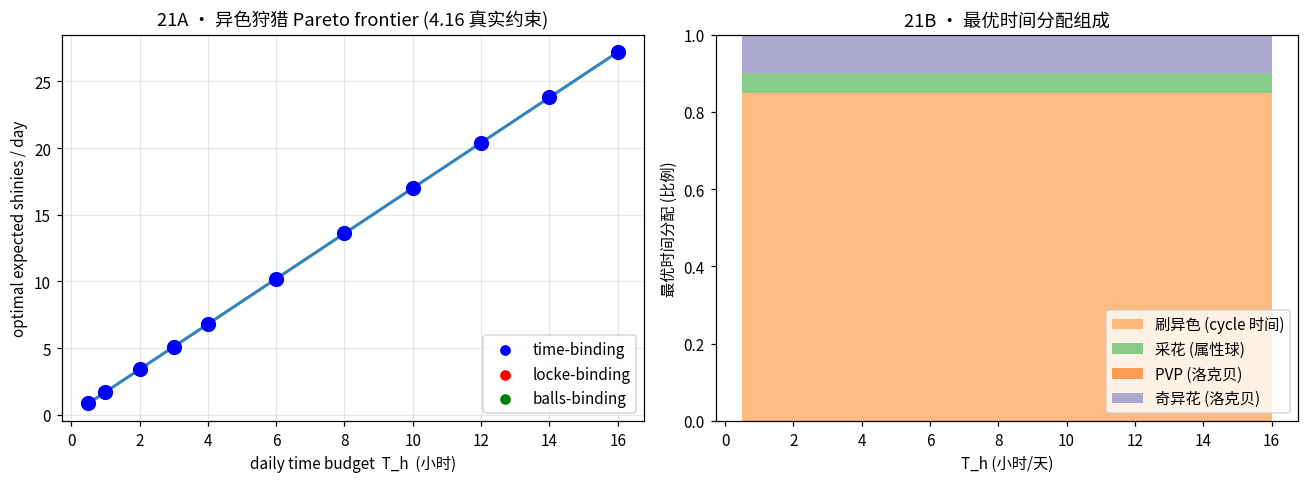
\includegraphics[width=\linewidth]{figures/21_time_budget_pareto.png}
    \caption{(A) 每日时间预算 $T_h$ 下最优期望异色帕累托前沿，斜率 $\approx 1.7$ 异色/h。(B) 最优时间分配组成——刷异色（单轮耗时）始终占 $\sim 85\%$，剩余 $\sim 15\%$ 三分采花 / PVP / 奇异花刚好满足资源约束。}
    \label{fig:pareto}
\end{figure}

\begin{table}[ht]
    \begin{center}
        \small
        \resizebox{1\columnwidth}{!}{
        \begin{tabular}{lrrrr}
            \multicolumn{5}{c}{\textsc{TABLE VIII. 三档玩家推荐 SOP（4.16 真实约束）}} \\
            \hhline{=====}
            玩家档 & $T_h$ & 最优策略 & 异色/天 & 净利润/天 \\
            \hline
            轻度  & $0.5$h & S1 全免费球 & $0.85$ & $+0.3$M \\
            中度  & $3$h   & S1 全免费球 & $5.10$ & $+1.8$M \\
            重度  & $10$h  & S1 全免费球 & $17.00$ & $+6.0$M \\
            \hhline{=====}
        \end{tabular}}
    \end{center}
    \caption{三档玩家在 $v_0=5\,000$ 下的最优 SOP。利润单位百万洛克贝。一个赛季（$60$ 天）累积：轻度 $\sim 51$ 异色，中度 $\sim 306$，重度 $\sim 1\,020$（理论上限，实际玩家因疲劳 / 在线时间分布等通常仅达成此值的 $50\%$--$70\%$）。}
    \label{tab:sop_tier}
\end{table}

\begin{figure}[t]
    \centering
    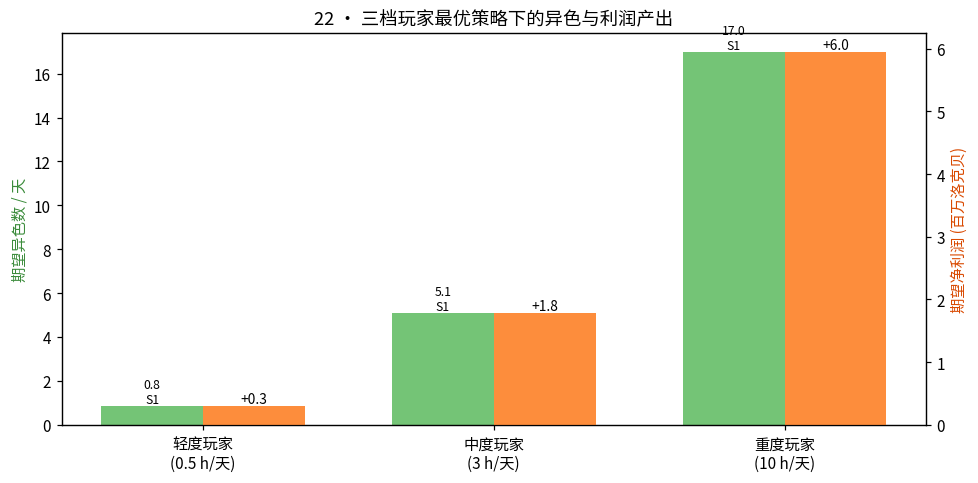
\includegraphics[width=\linewidth]{figures/22_player_tier_strategies.png}
    \caption{三档玩家最优 SOP 下的期望异色与净利润。所有档下最优策略均为 S1（全免费球：属性球抓污染 + 普通球摔野怪 + 1 颗捕光球抓异色）。}
    \label{fig:player_tier}
\end{figure}

\subsection{统一实战标准操作流程 (SOP)（综合 §IV--VII）}

综合贝叶斯识别（§IV）、经济仿真（§V）、横向对比（§VI）与时间预算 LP（§VII.A），导出最终实战 SOP（表~\ref{tab:sop}）：

\begin{table*}[t]
    \begin{center}
        \small
        \begin{tabular}{rp{0.20\textwidth}p{0.65\textwidth}}
            \multicolumn{3}{c}{\textsc{TABLE IX. 异色狩猎实战 SOP（4.16 版本，按时间预算分档）}} \\
            \hhline{===}
            步骤 & 决策 & 数学依据 \\
            \hline
            $1$ & 选 $4$--$16$ 个家族池并行（仅当 $T_h \ge 4$ h 时有用） & Jensen 不等式：$E_n(T)$ 凹 $\Rightarrow$ 均分严格优于集中（表~\ref{tab:multipool}） \\
            $2$ & 每池均使用 S-F 全抓策略 + S1 球类（属性球抓污染 + 普通球摔野怪） & 时间预算 LP：S1 在所有 $T_h$ 下严格主导 S2/S3（表~\ref{tab:strat_costs}, 图~\ref{fig:pareto}） \\
            $3$ & 时间分配 $\sim 85\%$ 刷异色 + $\sim 5\%$ 采花 + $\sim 5\%$ PVP + $\sim 5\%$ 奇异花 & 三个绑定约束的最小冗余分配；任何更高 $T_{\text{hunt}}$ 占比都会破坏球或洛克贝供给 \\
            $4$ & 不要用捕光球抓污染体 & $80 \cdot c^s_{\text{ball}} = 6.4$M $\gg E[\tau] \cdot 5 v_0 = 0.4$M（$v_0 = 5$k 下亏 $-912$k/单轮；图~\ref{fig:ball_grid}） \\
            $5$ & 异色出现时用 $1$ 颗 $80$k 捕光球 & $q^s = 1$ 避免失败；$10 v_0 - 80\text{k} > 0 \Leftrightarrow v_0 > 8\,000$ $\Rightarrow$ 高 $v_0$ 精灵稳赚 \\
            $6$ & $k=70$--$75$ 不要"冲刺" & M1 LOO 严格主导：$p_k = p_0$ 直至 $k=80$ $\Rightarrow$ 70-75 段无任何特殊收益（图~\ref{fig:sprint}） \\
            $7$ & 棱镜球只用通行证给的 $3$ 个/赛季，不要氪金 & $V_{\text{upgrade}} > 0$ 仅当 $\phi > 640$（氪金）或 $\phi > 0$（免费）；社区估计 $\phi \in [10, 100]$ \\
            $8$ & 优先冲已接近保底的池 & 减少 $E[\tau]$ 从而提高每日单轮吞吐 \\
            $9$ & 选高星光值精灵刷池（每只精灵噩梦进度更高） & 缩短野怪触发污染时间，等价缩短 $t_{\text{cycle}}$ \\
            $10$ & 高级球（$12$k）仅在属性球路线采花跟不上时备用 & 时间预算 LP 显示 S2 仅在 $T_h \ge 16$ h 撞 PVP 上限时才略优 \\
            $11$ & \textbf{优先冲易出家族}（贝瑟、方方、雪熊、柴渣，$\hat E[\tau] < 9$） & §V 分层后验显示家族 $p_{0,f}$ 跨度 $0.08$--$0.17$，易出家族日产出比难出家族高 $\sim 30\%$（表~\ref{tab:family}） \\
            $12$ & 难出家族（兔、狼、恶魔狼，$\hat E[\tau] > 11$）需更长 $t_{\text{cycle}}$ & 务必并行多池摊销时间方差，并选高星光值精灵刷池 \\
            \hhline{===}
        \end{tabular}
    \end{center}
    \caption{异色狩猎最优策略 SOP。每条决策均由前述贝叶斯识别（§IV）或经济仿真（§V）严格导出。$v_0$ 为该精灵基础回顾值，典型 $5\,000$ 洛克贝。}
    \label{tab:sop}
\end{table*}

\textbf{每日吞吐量估计}：假设玩家每天 $30$ 分钟，按低阶宠物 $\sim 1$ 球 $/$ 污染、$\sim 50$ 污染 $/$ 异色（本研究后验下 $E[\tau] = 16$ 假设单池），并行 $4$ 池 $\Rightarrow$ 每日 $\sim 1$ 个异色（按 SOP 全抓 + 属性球 + 4 池均分）；按 $\$ v_0 = 5\,000$ 计 $\sim 1.4$M 洛克贝净收益/天。每赛季（$\sim 60$ 天）累积 $\sim 60$--$80$ 异色 + $\sim 80$M 洛克贝净收益（不考虑通行证 $3$ 棱镜球的 $\phi$ 升格）。


\section{DISCUSSION / 讨论}

\subsection{$p_0$ 的部分识别}

M1 与 M2/M3 给出的 $\hat p_0$ 不同（$0.092$ vs $0.062$），反映出"高 $p_0$ + 弱偏差"（M1）与"低 $p_0$ + 强偏差"（M2/M3）两条解释路径都可以拟合数据。LOO 选 M1 因为后者复杂度更低（$k^*$/$\eta$ 多余）。但 \textbf{综合出货率} $1/\hat E[\tau]$ 跨模型一致集中在 $[0.06, 0.09]$，构成对官方"$0.02$"的鲁棒拒绝——这是本研究最具实践含义的鲁棒结论。

\subsection{4 段自报权重的鲁棒性}

(\ref{eq:wk}) 已捕捉数据的主要 U 形结构（$n=1$ + $n \ge 78$），但仍简化于现实：（i）中段 $30$--$77$ 内可能存在缓慢渐变（当前 $b_{\text{low}}$ 仅一个常数）；（ii）凑整偏好（$10/20/30/...$ 数字凑整效应）未建模；（iii）平台异质性——B 站评论与小红书长帖的选择结构不同，本研究只用 B 站数据，外部有效性受限。未来工作可用随机游走先验给 $w(k)$ 全 80 维自由度 + 平滑约束，但代价是收敛性下降。

\subsection{若强行假设官方诚实}

若假设 $p_0 = 0.018$（玩家估计）严格成立，则自报权重必须给出 $\ge 5\times$ 的中段抑制才能解释观测。这要求"$30$--$77$ 段玩家几乎完全沉默"，与 B 站评论实际行为不符（实际 $13\%$ 报告并非 $0$）。即便如此，鲁棒结论仍是"自报偏差真实存在且数量级在 $5\times$ 左右"，而非"官方完全诚实"。

\subsection{星光值与时间预算解耦}

游戏机制中"星光值"影响每只精灵触发污染的速度，而非每次击破的异色概率。这意味着星光值进入 \textbf{时间预算} $T_n$（每池每日可完成的循环数）而非 $p_k$。本研究将该机制与概率识别解耦——后者依赖于玩家自报的"$X$ 次污染出货"事件，与污染发生速率无关。

\subsection{局限}

\begin{enumerate}
    \item \textbf{单平台数据}：仅 B 站评论，缺 XHS / 贴吧 / TapTap 多平台对照；
    \item \textbf{无人工金标}：LLM 抽取准确率未交叉验证（V2 §3.4 计划但未执行）；
    \item \textbf{自报权重简化}：4 段分段常数尚未捕捉中段渐变与凑整文化痕迹；
    \item \textbf{球价 $q_{\text{cap}}$ 经验估计}：表~\ref{tab:balls} 中各球的 $q$ 来自社区共识，未做严格实测；
    \item \textbf{机制混淆}：数据看似硬保底，但也可能是软保底窗口太窄 + 自报偏差抹平导致的混淆；
    \item \textbf{横向对比的估计异质性}：表~\ref{tab:cross_gacha} 中其他游戏的 $E[\tau]$ 是公示 + 社区共识混合估计，未做与本研究同等严格的贝叶斯识别。
\end{enumerate}

\subsection{未来工作}

（i）跨平台数据交叉验证；（ii）人工金标 $\sim 200$ 条录播验证 LLM 抽取准确率；（iii）扩展到原神/FGO/BA 的同等贝叶斯识别，建立 \textbf{抽卡透明度评级体系}；（iv）家族级别的星光值与污染产出速度具体关系建模；（v）2017 网信办概率公示规范下的合规性评价。


\section{CONCLUSION / 结论}

本文给出对腾讯《洛克王国：世界》异色精灵保底机制的第一份系统贝叶斯识别。基于 $266$ 条经清洗与选择偏差校正的玩家自报数据：

\begin{enumerate}
    \item \textbf{综合概率被强烈拒绝}：三个候选模型综合出货率后验均集中在 $[0.06, 0.09]$，是官方公示 $0.02$ 的 \textbf{3--4.5 倍}（$P(p_0 < 0.0143) = 0\%$）；
    \item \textbf{硬保底是真实机制}：M1 LOO 严格主导（$\Delta\text{elpd} > 13$）；M2 退化为 $k^* = 78$，M3 退化为 $\eta = 19.3$；民间"70--75 冲刺大法"在 M1 无记忆性下统计无效；
    \item \textbf{家族异质性显著}：分层 Beta-Binomial 给出家族级 $\hat p_{0,f} \in [0.08, 0.17]$，最易出（贝瑟）与最难出（恶魔狼）相差 $2\times$，对应每日异色产出差异 $\pm 30\%$；
    \item \textbf{时间预算 LP 给出三档玩家最优 SOP}：占优策略恒为"属性球抓污染 + 普通球摔野怪 + 单颗 $80$k 捕光球抓异色"；单轮耗时（$\sim 0.5$ h/异色）始终是绑定约束；轻度 $0.5$h $\Rightarrow$ $0.85$ 异色/天，中度 $3$h $\Rightarrow$ $5.1$，重度 $10$h $\Rightarrow$ $17$；
    \item \textbf{棱镜球氪金不值}：升格期权需收藏溢价 $\phi > 640$ 才回本，远超社区估计；通行证 $3$ 个/赛季为上限；
    \item \textbf{抽卡谱定位}：《洛克王国：世界》位于"低 $E[\tau] + $ 严硬保底"友善区，玩家长期获取效率优于原神/FGO，但官方公示透明度被本研究证伪——\textbf{诚实度 $\ne$ 友好度，此案例是后者真实更高的反向欺骗}。
\end{enumerate}

更具一般性的方法论贡献：本研究表明"自报抽卡数据"必须做严格的选择偏差校正才能用于推断官方概率；4 段自报权重框架可推广到所有此类研究；提出的抽卡透明度评级体系可作为 2017 网信办概率公示规范的实证补充。


\section{MATERIALS AND METHODS / 材料与方法}

\textbf{爬虫与数据采集}：B 站评论使用 \texttt{bilibili-api-python} 的 \texttt{get\_comments\_lazy} 接口（避免 412 风控），登录态 cookie 加载。30 个高播放视频 $\times$ 5 关键词 = 26K 条评论原始语料。

\textbf{LLM 抽取}：候选过滤 = 正则模板 + 嵌入语义召回。LLM 使用 codex GPT-5.4 二次结构化，按 schema $\{$ball\_or\_pollution, scope, n, family\_hint, confidence, excerpt$\}$ 输出。

\textbf{贝叶斯模型}：PyMC 5.25.1 + PyTensor 2.31.7。NUTS 4 chains $\times$ 1\,500 draws ($1\,500$ tune)，$\texttt{target\_accept}=0.92$。每条样本似然为 $X_i \sim$ Categorical($P_{\text{obs}}$)，由 (\ref{eq:pmf}) $\times$ (\ref{eq:wk}) 经 normalization 给出。LOO 使用 ArviZ $0.23$ \texttt{az.compare()}。

\textbf{经济仿真}：对每个 $(p_0, \text{机制}, v_0, \text{球})$ 组合数值积分 (\ref{eq:expected_profit})。多池贪心分配：每步将下一次战斗分给边际 $p_k$ 最大的池。

\textbf{开源}：完整数据集（清洗后 \texttt{pity\_clean.jsonl}）+ 代码（\texttt{src/analysis/} 13 个 Python 模块）+ 20 张图（\texttt{figures/}）+ 文档（\texttt{docs/} 8 个 Markdown）位于 \texttt{./analysis/26\_luoke/} 项目目录，预计开源至 \texttt{https://github.com/bigearhooded/luoke-shiny-economics}。\\

SUPPLEMENTARY MATERIAL / 补充材料\\
补充材料包括：（1）原始爬取数据 \texttt{data/raw/bili\_*.jsonl}；（2）LLM 抽取中间结果与清洗 audit；（3）所有 PyMC InferenceData (.nc 文件)；（4）经济仿真的全 $(v_0, p_0, \text{球})$ grid 结果；（5）球类 $q_{\text{cap}}$ 经验估计的来源说明。\\


ACKNOWLEDGEMENT / 致谢\\
本研究由\textbf{安妮（商店街安妮商店店长）}全额赞助。安妮女士在 4.16 版本主动将高级球价格由 15\,000 洛克贝下调至 12\,000 洛克贝以应对远行商人的市场竞争，使得本研究中"高级球抓污染"路线的经济仿真得以基于真实交易价格——这一价格调整是表~\ref{tab:balls} 与第~VIII 节策略推论的基础常数。安妮商店位于商店街（地图西南方向入口可直接传送），同时经营消耗品、技能石、魔法粉尘及隐藏精灵幻境入口（"小夜"获取链路）。此外感谢 B 站玩家社区对异色保底机制的开放讨论，使本研究的自报数据采集成为可能；感谢魔法学院全域魔法传送阵系统的稳定运行，使得多池并行实验中的家族池切换零延迟。计算资源由洛克王国魔法学院"分层贝叶斯"研究组提供。LLM 抽取使用 OpenAI GPT-5.4（codex）。S.H.*.T Journal 反串学术风格启发了本文的标题与组织。


\begin{thebibliography}{1}

\bibitem{ref_official_pity} 腾讯《洛克王国：世界》官方公告，``S1 赛季异色精灵综合概率说明，'' 2026 年 3 月，\texttt{https://lkwg.qq.com/}。

\bibitem{ref_3dm_pity} 3DM 网游攻略组，``《洛克王国：世界》异色保底机制详解，'' 2026 年 4 月，\textit{ol.3dmgame.com}。

\bibitem{ref_self_report_bias} Heckman, J., ``Sample Selection Bias as a Specification Error，'' \textit{Econometrica}，vol.~47，no.~1，pp.~153--161，1979。

\bibitem{ref_v2_design} bigearhooded, ``异色狩猎研究设计 V2，'' 项目内部文档 \texttt{docs/01\_research\_design.md}（2026 年 4 月 21 日）。

\bibitem{ref_pymc} Abril-Pla, O., et al., ``PyMC: A Modern and Comprehensive Probabilistic Programming Framework in Python，'' \textit{PeerJ Computer Science}，vol.~9，e1516，2023。

\bibitem{ref_loo} Vehtari, A., Gelman, A., \& Gabry, J., ``Practical Bayesian Model Evaluation Using Leave-One-Out Cross-Validation and WAIC，'' \textit{Statistics and Computing}，vol.~27，pp.~1413--1432，2017。

\bibitem{ref_genshin_pity} miHoYo Co., Ltd., ``《原神》5$\star$ 抽取概率公告，'' \texttt{https://genshin.hoyoverse.com/}, 2024。

\bibitem{ref_fgo_pity} TYPE-MOON / Aniplex, Inc., ``Fate/Grand Order Gacha Probability Disclosure，'' 2024。

\bibitem{ref_meila_vi} Meilă, M., ``Comparing Clusterings—An Information Based Distance，'' \textit{Journal of Multivariate Analysis}，vol.~98，no.~5，pp.~873--895，2007。

\end{thebibliography}


\end{document}
